\begin{figure*}[h]
\centering
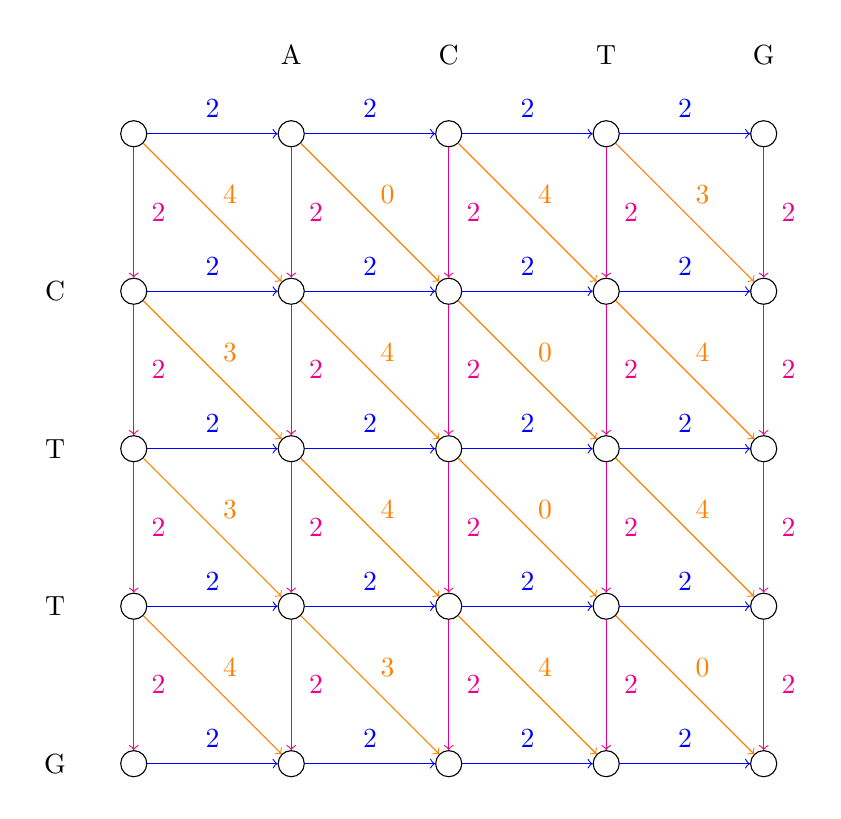
\begin{tikzpicture}[shape=circle,auto]
    \node[draw] (A) at (0,0) {};
    \node[draw] (B) at (2,0) {};
    \node[draw] (C) at (4,0) {};
    \node[draw] (D) at (6,0) {};
    \node[draw] (E) at (8,0) {};
    \node[draw] (F) at (0,2) {};
    \node[draw] (G) at (2,2) {};
    \node[draw] (H) at (4,2) {};
    \node[draw] (I) at (6,2) {};
    \node[draw] (J) at (8,2) {};
    \node[draw] (K) at (0,4) {};
    \node[draw] (L) at (2,4) {};
    \node[draw] (M) at (4,4) {};
    \node[draw] (N) at (6,4) {};
    \node[draw] (O) at (8,4) {};
    \node[draw] (P) at (0,6) {};
    \node[draw] (Q) at (2,6) {};
    \node[draw] (R) at (4,6) {};
    \node[draw] (S) at (6,6) {};
    \node[draw] (T) at (8,6) {};
    \node[draw] (U) at (0,8) {};
    \node[draw] (V) at (2,8) {};
    \node[draw] (W) at (4,8) {};
    \node[draw] (X) at (6,8) {};
    \node[draw] (Y) at (8,8) {};
    
    \draw (2,9) node{A};
    \draw (4,9) node{C};
    \draw (6,9) node{T};
    \draw (8,9) node{G};
    \draw (-1,0) node{G};
    \draw (-1,2) node{T};
    \draw (-1,4) node{T};
    \draw (-1,6) node{C};

    \draw (A) edge[blue, ->] node {2} (B);
    \draw (B) edge[blue, ->] node {2} (C);
    \draw (C) edge[blue, ->] node {2} (D);
    \draw (D) edge[blue, ->] node {2} (E);
    \draw (F) edge[blue, ->] node {2} (G);
    \draw (G) edge[blue, ->] node {2} (H);
    \draw (H) edge[blue, ->] node {2} (I);
    \draw (I) edge[blue, ->] node {2} (J);
    \draw (K) edge[blue, ->] node {2} (L);
    \draw (L) edge[blue, ->] node {2} (M);
    \draw (M) edge[blue, ->] node {2} (N);
    \draw (N) edge[blue, ->] node {2} (O);
    \draw (P) edge[blue, ->] node {2} (Q);
    \draw (Q) edge[blue, ->] node {2} (R);
    \draw (R) edge[blue, ->] node {2} (S);
    \draw (S) edge[blue, ->] node {2} (T);
    \draw (U) edge[blue, ->] node {2} (V);
    \draw (V) edge[blue, ->] node {2} (W);
    \draw (W) edge[blue, ->] node {2} (X);
    \draw (X) edge[blue, ->] node {2} (Y);

    \draw (F) edge[magenta, ->] node {2} (A);
    \draw (G) edge[magenta, ->] node {2} (B);
    \draw (H) edge[magenta, ->] node {2} (C);
    \draw (I) edge[magenta, ->] node {2} (D);
    \draw (J) edge[magenta, ->] node {2} (E);
    \draw (K) edge[magenta, ->] node {2} (F);
    \draw (L) edge[magenta, ->] node {2} (G);
    \draw (M) edge[magenta, ->] node {2} (H);
    \draw (N) edge[magenta, ->] node {2} (I);
    \draw (O) edge[magenta, ->] node {2} (J);
    \draw (P) edge[magenta, ->] node {2} (K);
    \draw (Q) edge[magenta, ->] node {2} (L);
    \draw (R) edge[magenta, ->] node {2} (M);
    \draw (S) edge[magenta, ->] node {2} (N);
    \draw (T) edge[magenta, ->] node {2} (O);
    \draw (U) edge[magenta, ->] node {2} (P);
    \draw (V) edge[magenta, ->] node {2} (Q);
    \draw (W) edge[magenta, ->] node {2} (R);
    \draw (X) edge[magenta, ->] node {2} (S);
    \draw (Y) edge[magenta, ->] node {2} (T);

    \draw (F) edge[orange, ->] node {4} (B);
    \draw (G) edge[orange, ->] node {3} (C);
    \draw (H) edge[orange, ->] node {4} (D);
    \draw (I) edge[orange, ->] node {0} (E);
    \draw (K) edge[orange, ->] node {3} (G);
    \draw (L) edge[orange, ->] node {4} (H);
    \draw (M) edge[orange, ->] node {0} (I);
    \draw (N) edge[orange, ->] node {4} (J);
    \draw (P) edge[orange, ->] node {3} (L);
    \draw (Q) edge[orange, ->] node {4} (M);
    \draw (R) edge[orange, ->] node {0} (N);
    \draw (S) edge[orange, ->] node {4} (O);
    \draw (U) edge[orange, ->] node {4} (Q);
    \draw (V) edge[orange, ->] node {0} (R);
    \draw (W) edge[orange, ->] node {4} (S);
    \draw (X) edge[orange, ->] node {3} (T);
\end{tikzpicture}
\end{figure*}
%%% Local Variables:
%%% mode: latex
%%% TeX-master: "../rapport"
%%% End:
